\documentclass[a4paper]{article}
\usepackage[affil-it]{authblk}
%\usepackage[backend=bibtex,style=numeric]{biblatex}
\usepackage{graphicx} % Required for inserting images
\usepackage{caption}

\usepackage{ctex}
\usepackage{epstopdf}
\usepackage{amsfonts,amssymb}
\usepackage{tikz}
\usetikzlibrary{chains}
\usepackage{listings}
\usepackage{xcolor}
\usepackage{float}
\usepackage{hyperref}
\usepackage{bookmark}
\usepackage{subfig}
\usepackage{listings,matlab-prettifier} % MATLAB 美化包
% \lstset{
%         style=Matlab-editor,
%         numbers      = left,
%         frame        = single,
% }
\usepackage{amsmath}
\usepackage{chngcntr}
\counterwithout{equation}{section}
\counterwithout{figure}{section}

\usepackage{geometry}
\geometry{margin=1.5cm, vmargin={0pt,1cm}}
\setlength{\topmargin}{-1cm}
\setlength{\paperheight}{29.7cm}
\setlength{\textheight}{25.3cm}


\begin{document}
% =================================================
\title{NA programming homework \#2}

\author{陈澎 Chen Peng 3220103443
  \thanks{Email: \texttt{cpzju@zju.edu.cn}}}
\affil{Xinji 2201, Zhejiang University }


\date{\today}

\maketitle

% ============================================
\section*{Problem A}


\section*{Problem B}
Complie and run the program \verb|B.cpp|. Its output is the Newton interpolation polynomial of each situations.
It is shown as below.
\begin{lstlisting}[breaklines=true]
when n=2, p(x)=1-0.03846154*x^2
when n=4, p(x)=1+2.775558e-017*x-0.1710875*x^2+3.469447e-018*x^3+0.00530504*x^4
when n=6, p(x)=1-5.551115e-017*x-0.3513637*x^2+0.0335319*x^4-8.673617e-019*x^5-0.0008406327*x^6
when n=8, p(x)=1-1.387779e-017*x-0.5281214*x^2-9.714451e-017*x^3+0.09818753*x^4+8.673617e-018*x^5-0.006580161*x^6+0.0001374446*x^8
\end{lstlisting}

Use matlab to plot each $p(x)$ and the function $\dfrac{1}{1+x^2}$ in $[-5,5]$. The image is Fig.\ref{fig1}, which is drawn by \verb|B_plot.m|.
From the Fig.\ref{fig1}, we can find that it has wide oscillations no matter how large the $n$ is.
\begin{figure}[htbp]
  \centering
  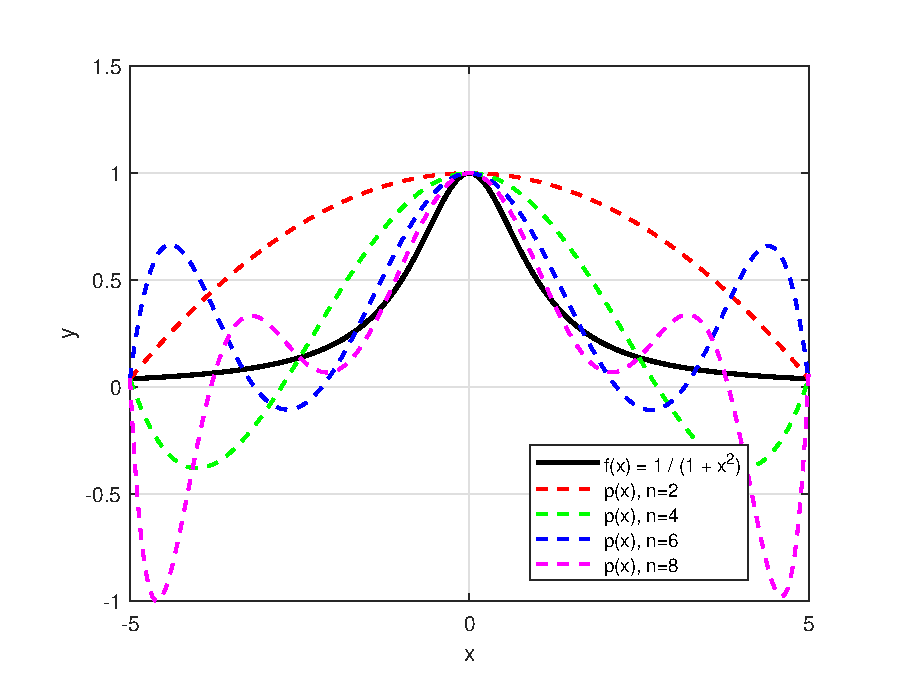
\includegraphics[width=0.6\textwidth]{images/B_pic.eps}
  \renewcommand{\figurename}{Fig.}
  \caption{Comparison of interpolating Polynomials and Function $f(x)=\dfrac{1}{1+x^2}$}
  \label{fig1}
\end{figure}

\section*{Problem C}
Complie and run the program \verb|C.cpp|. Its output is the Newton interpolation polynomial of each situations.
\begin{lstlisting}[breaklines=true]
when n=5, p(x)=1-1.110223e-016*x-3.542983*x^2+4.440892e-016*x^3+2.746498*x^4
when n=10, p(x)=0.7308217-7.392743e-016*x-4.811625*x^2+5.095772e-015*x^3+12.61929*x^4-2.700829e-014*x^5-14.00244*x^6+3.820127e-014*x^7+5.512772*x^8-1.573687e-014*x^9
when n=15, p(x)=1+2.553513e-015*x-17.36407*x^2-2.664535e-014*x^3+149.0269*x^4+2.131628e-013*x^5-646.8639*x^6+1.080025e-012*x^7+1510.606*x^8+1.818989e-012*x^9-1927.183*x^10+1264.416*x^12+2.842171e-013*x^13-333.619*x^14
when n=20, p(x)=0.9624097-2.545115e-015*x-16.54218*x^2-5.953458e-015*x^3+165.4582*x^4+7.125567e-013*x^5-960.8247*x^6+1.237559e-011*x^7+3379.017*x^8-2.322308e-011*x^9-7413.453*x^10+3.365297e-011*x^11+10195.47*x^12-2.58698e-011*x^13-8534.894*x^14+4.561769e-011*x^15+3973.165*x^16-1.688679e-011*x^17-788.3263*x^18+3.307113e-012*x^19
\end{lstlisting}

Use matlab to plot each $p(x)$ and the function $\dfrac{1}{1+25x^2}$ in $[-1,1]$. The image is Fig.\ref{fig2}, which is drawn by \verb|C_plot.m|.

From Fig.\ref{fig2}, we can find that the larger the $n$, the better the approximation. It is free of the wide oscillations in the previous assignment.
\begin{figure}[htbp]
  \centering
  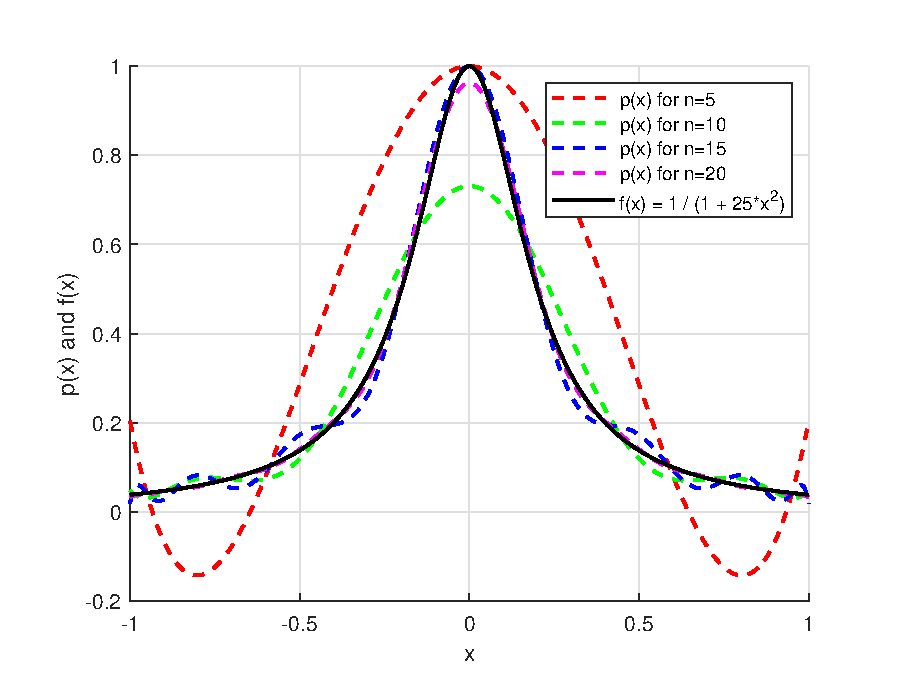
\includegraphics[width=0.6\textwidth]{images/C_pic.eps}  
  \renewcommand{\figurename}{Fig.}
  \caption{Comparison of interpolating Polynomials and Function $f(x)=\dfrac{1}{1+25x^2}$}
  \label{fig2}
\end{figure}

\section*{Problem D}
Complie and run the program \verb|D.cpp|. Its output is the anwser. 
\begin{lstlisting}[breaklines=true]
  (a)p(x)=75*x+7.161908*x^2-10.09531*x^3+5.508121*x^4-1.538296*x^5+0.2430412*x^6-0.02187567*x^7+0.00104059*x^8-2.022363e-005*x^9
  p'(x)=75+14.32382*x-30.28593*x^2+22.03248*x^3-7.691478*x^4+1.458247*x^5-0.1531297*x^6+0.008324722*x^7-0.0001820127*x^8
  Speed at t=10s is p'(10)=48.38174feet/s
  (b) max speed is 119.4173feet/s at t=12.37184s. it exceeds the speed limit.
  \end{lstlisting}

I use a simple grid search over the interval to find 
points where the derivative is close to zero, indicating critical points in order to evaluate the extrema.


\section*{Problem E}
Complie and run the program \verb|D.cpp|. Its output is the Newton interpolation polynomial.
\begin{lstlisting}[breaklines=true]
(a)For sp1, sp1(x)=6.67-43.01266*x+16.28546*x^2-2.115118*x^3+0.1282809*x^4-0.00371557*x^5+4.147705e-005*x^6
For sp2, sp2(x)=6.67-5.85018*x+2.982271*x^2-0.4242825*x^3+0.02658578*x^4-0.0007774732*x^5+8.676802e-006*x^6
(b)For sp1, sp1(43)=14640.26
For sp2, sp2(43)=2981.477
\end{lstlisting}
\subsection*{(a)}
The average weight curve of Sp1 and Sp1 predicted by Newton's formula is as Fig.\ref{fig3} shown, which is drawn by \verb|E_plot.m|.
\begin{figure}[htbp]
  \centering
  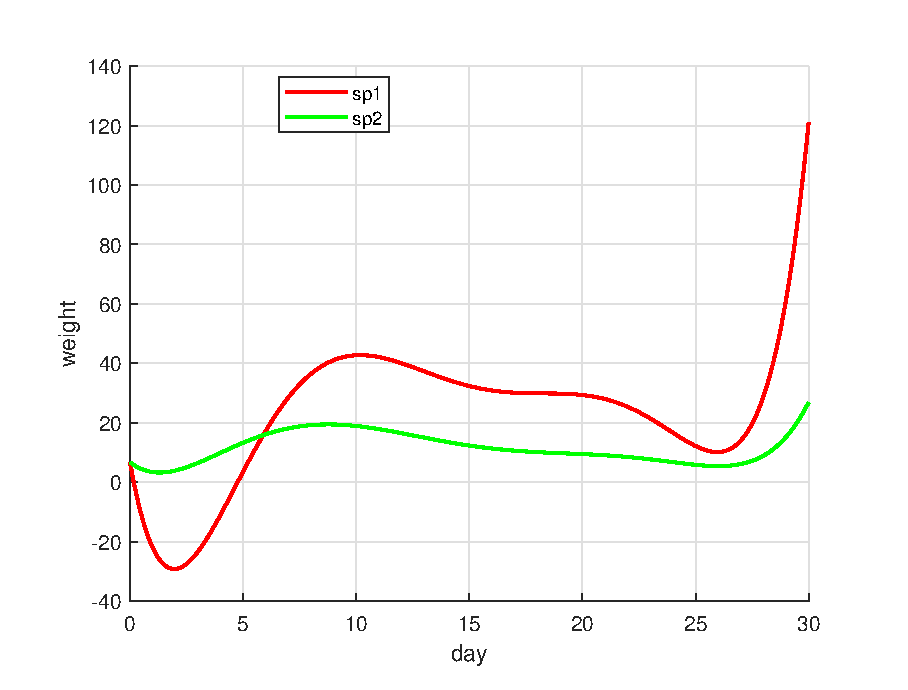
\includegraphics[width=0.6\textwidth]{images/E_pic.eps}  
  \renewcommand{\figurename}{Fig.}
  \caption{Predicting weight curve of wo samples of larvae in 30 days}
  \label{fig3}
\end{figure}

\subsection*{(b)}
Use the formula by (a) to predict the average weight of the two samples of larvae after another 15 days. 
For Sp1, the predicted average weight is 14640.26 at day 43. For Sp2, the predicted average weight is 2981.477 at day 43.

So the two samples of larvae won't die after another 15 days according to the prediction.

Actually, the prediction is not accurate enough. So the prediction maybe wrong. 

\section*{Problem F}
Complie and run the program \verb|F.cpp|. It generates the data of Bezier curves'coordinates and import them correspondingly into \verb|data_10.txt|, \verb|data_400.txt| and \verb|data_160.txt|. 

When choosing consecutive marker points, I choose the points evenly on the premise of obtaining two points where $x=0$ in order to approximate the tips of the heart. Besides, I add the consecutive marker points $\mathbf{p}_{m+1}=\mathbf{p}_{0}$ to form closed curves.
\begin{figure}[htbp]
  \centering
  \subfloat[Scatter Plot of $m=10$]
  {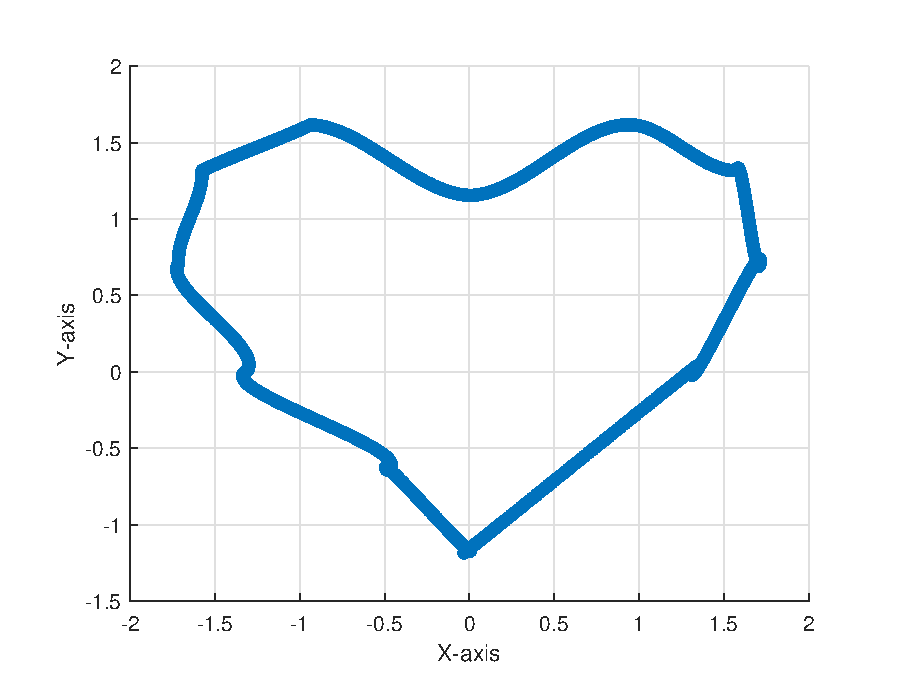
\includegraphics[width=0.4\textwidth]{./images/F_pic_10.eps}\label{fig4a}}  
  \subfloat[Scatter Plot of $m=40$]
  {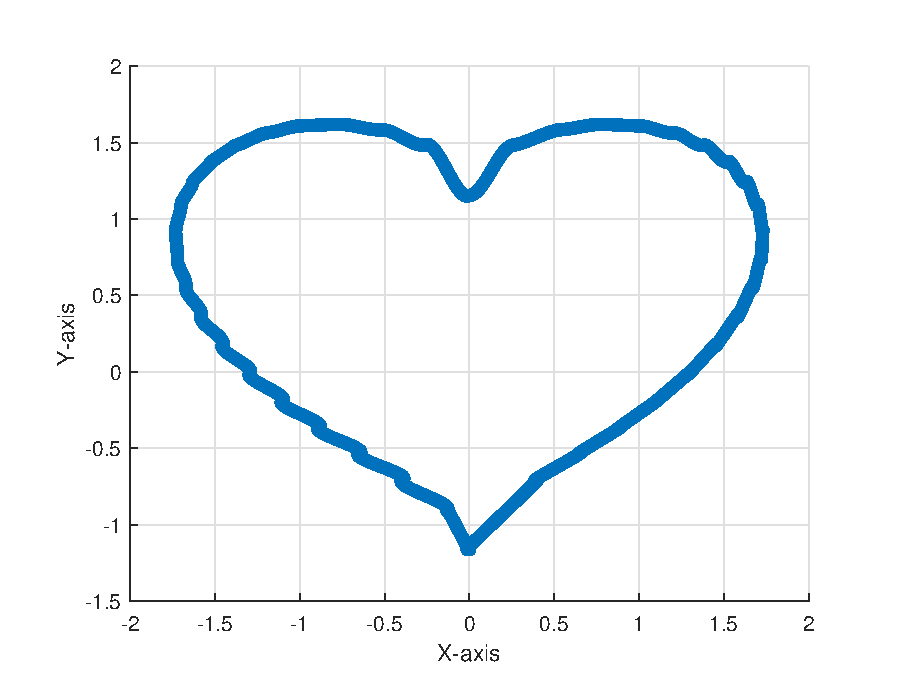
\includegraphics[width=0.4\textwidth]{./images/F_pic_40.eps}\label{fig4b}}\\
  \subfloat[Scatter Plot of $m=160$]
  {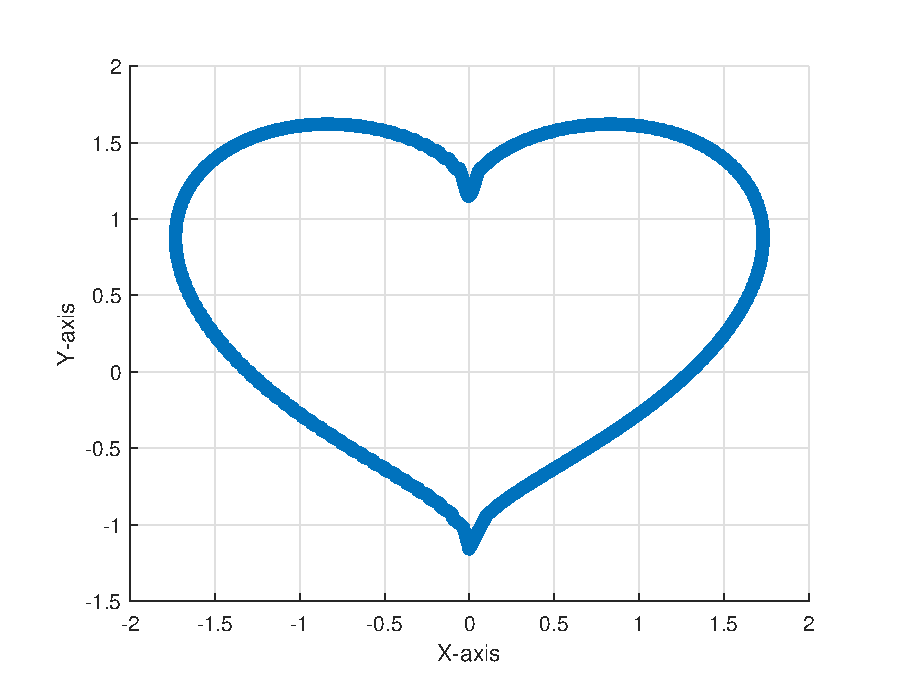
\includegraphics[width=0.4\textwidth]{./images/F_pic_160.eps}\label{fig4c}}
  \renewcommand{\figurename}{Fig.}
  \caption{cubic Bezier curves approximating the heart}
  \label{fig4}
\end{figure}

\end{document}